\chapter*{Abstract}

A szakdolgozatban fűtési rendszerek modell-prediktív szabályzásának lehetőségeit vizsgálom Matlab Simulinkben. %Szimulációval
Végighaladok az MPC tervezés lépésein, a tervezést és a validálást is szimulált szakaszmodellen végzem. A szakaszmodellt a fűtési rendszer és a szoba alkotja, a fűtés hője a szobából külső falon távozik a környezet felé. Az állandósult állapotban szükséges fűtési teljesítményt képlettel számítom, ebből kapható a beavatkozó jel egy adott teljesítményigényhez. A hőkapacitásokat és hőátadási, hővezetési tényezőket Simscape modell tartalmazza%(\ref{table_heater_parameters}. és \ref{table_house_parameters}. táblázat)
, meghatározva a szakasz dinamikáját. Megvizsgálom az MPC predikciós horizontjának, költségfüggvényének illetve mintavételi idejének hatását a zárt szabályzási kör viselkedésére.  %tranziens viselkedését
%A szimulációhoz felállított modellhez számításokra is szükség van,
%Állandósult állapotra felírt képlet adja a szükséges fűtési teljesítményt

A tervezési lépéseket ezután valós, fizikai modellen is elvégzem, így látható lesz, hogy egy kész házra, vagy annak egy részére mennyi munkával jár a szabályzó beállítása. Ha a modellezésre, hangolásra fordított idő megtérül, azaz komfortnövekedéssel, illetve az üzemeltetési költségek csökkenésével jár, akkor a funkciókat akár az iContrALL okosház platformba is be lehet illeszteni.
%a módszer pénzbeli haszonnal is kecsegtet.

 % rendezzük a  \ref{eq_holeadas4}-t alpha-ra!

%a beavatkozók, a mérhető zavarások és a hibajel függvényében.
% kapom, ez méretezéshez és költségek számításához használható. 

\chapter{Bevezetés}

%Van egy ház
%
%Van egy fűtési rendszere
%
%Vannak szabályozható szelepek a szobákban
%
%Hogyan szabályozzuk?


Európa / Magyarország energiafelhasználásának x százalékát az épületek adják, így a kibocsátás x százaléka is innen származik.
%A szmogot, a nagy szállópor-koncentrációt számos vidéki városban az elavult fűtési rendszerek okozzák.
Ezek a tényezők életminőségünkre is kihatással vannak, ezért manapság számos újépítésű lakó- vagy irodaháznál figyelembe veszik az energiahatékonysági szempontokat. A törvények előírják energetikai tanúsítvány készítését szerte az Unióban. Számos megtakarítási forma már régóta él a köztudatban, ezek például a szigetelés, az ablakcsere, a háztartási gépek cseréje. Az ágazat úttörői az építészek, többnyire a szerkezetek tervezésénél veszik figyelembe a fenti szempontokat.
%Az üzemeltetési időszakra viszont kevesebb figyelem kerül, szerencsére manapság már a teljes élettartamra vetített költséget is figyelembe szokás venni.
Az épületgépészeti rendszerek automatizálása viszont kevesebb embernek fontos, lakóházakban elterjedtek az egyszerű termosztátok.
%Irodaházakban van piaca bonyolultabb eljárásoknak.

%különben lakókörnyezetünkben
%A környezetvédelem és a költséghatékonyság 



Fel kell állítani egy paraméterezhető ház- és fűtőtest modellt, hogy annak paramétereit az energetikai tanúsítványból le tudjuk olvasni, ezzel egy közelítő modelljét megkapjuk a háznak. Ezen modell alapján már identifikáció nélkül is lehetséges a szabályzás, így a telepítés ideje lecsökkenthető, az identifikációt potenciálisan elrontó hatások pedig nem jelentkeznek. Ugyanis megbízható identifikáció nagyon sok időt venne igénybe.\footnote{Thieblemont state of art weather fc MPC-ben szót ejt róla}(Adaptív szabályzást egyelőre nem használok.)





A fűtőtestek feladata, hogy az adott szobában teljesítményt szolgáltassanak / (hőt\footnote{A hő mértékegysége \si{\joule}, a teljesítményé [\si{\watt}]~=~[\si[per-mode=fraction]{\joule\per\second}]}) adjanak le. A leadott teljesítmény növeli a levegő és az épületszerkezet hőjét (\ref{eq_holeadas4}. egyenlet). A levegőnek, padlónak, falaknak tömegüknél és fajhőjüknél fogva mind-mind van egy hőtároló képességük (\ref{table_house_parameters}. táblázat), így ezen elemek hőmérséklete nem változhat ugrásszerűen, hanem egy bizonyos idő alatt tudnak feltöltődni vagy hőenergiájukat leadni. %Mindezekben villamosmérnöki szemszögből felfedezhetjük az analógiát a villamos hálózatokkal.

A hasonlóság nem véletlen a villamos hálózatokkal. Felfedezhető, hogy a hő\textbf{áram}ot a hőmérsékletkülönbség hozza létre, nagysága pedig fordítottan arányos a hővezetési tényezővel. 


Munkámban elsősorban a különböző fűtési típusok közti különbségeket szeretném megvizsgálni. A ház modelljét először adottnak venném, az eltérést pedig a különböző fűtési módok jelentenék.
Azaz megpróbálom felírni a környezet belső hőmérsékletre való ráhatását, eztán pedig modellezem többféle fűtőtest viselkedését.

Ehhez először áttekintettem a hőátadás lehetséges formáit és forrásait.
Ezután fűtőtestek modelljét állítom fel.

Helyi szabályzást valósítok meg, \cite[118.~o.]{Herz} szerint.

Méretezés, stacioner állapot, kazánok \cite[235.~o.]{Herz} szerint. kazánok hatásfoka, túlméretezése. 313.o: fűtőtest mérés, be kell helyettesíteni.


\pagebreak

 Arra jutottam, hogy ha a levegő hőmérsékletére szabályzok, akkor az abba beleszóló tényezőket veszem sorra:
\begin{itemize}[noitemsep,topsep=0pt,parsep=0pt,partopsep=0pt]
	\item konvektív hőátadás: a felszín közelében felmelegedett levegő áramlani kezd
	\item radiatív hőátadás: sugárzással kibocsátott energia a környezetbe
\end{itemize}

\begin{figure}[h]
	\centering
	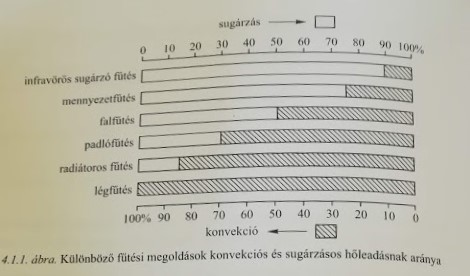
\includegraphics[width=8cm]{figures/konvrad}
	\caption{Alacsony hőmérsékletű fűtés és magas hőmérsékletű hűtés c. könyv ábrája}
		%\footnote{Jan Babiak, rehva Guidebook No.7}
\end{figure}


A levegő hőmérsékletére ezek a következőképp hatnak a leginkább:
\begin{itemize}[noitemsep,topsep=0pt,parsep=0pt,partopsep=0pt]
	\item a fűtőtestek konvektív és radiatív hőátadással is melegítik a környezetet
	\item a radiatív energiát a tárgyak, falak nyelik el, amik ezáltal felmelegszenek (mintegy kapacitásként lesz egy hőtároló tömeg, ami a fűtés kikapcsolásával fenntartja a hőmérsékletet / lassítja a hűlést)
	\item a fűtetlen falfelületek hűtik a szobát (külső hőmérséklet befolyása)
\end{itemize}

Így a kezdeti modellben azzal a feltételezéssel élek, hogy ezen kívül más hatás nem lép fel.

A modellben feltételezem, hogy a fűtőtest felületi hőmérsékletével tudunk beavatkozni. A modellben paraméter a fűtőtestek hőátadási tényezője és felülete. Zavarásként (?) hat a külső hőmérséklet értéke, amit mérni is tudunk. Kimenet a belső hőmérséklet (térben konstansnak véve azt / átlagolva a szoba levegőjére)

A modell felírásához a fűtőtest tulajdonságain kívül szükség van a szobában található levegő mennyiségére is. A zavarás hatását is fel kell írni, azaz hogy egy külső hőmérsékletváltozás hogyan jelenik meg a kimeneten. (Célszerű itt egy átviteli függvényt felírni először, szuperpozíciószerűen. A zavarás viszont nem a modell bemenetén és nem is a kimenetén hat.)

A felírandó átviteli függvények:

\begin{itemize}[noitemsep,topsep=0pt,parsep=0pt,partopsep=0pt]
	\item levegő felmelegedése konstans külső hőmérsékletet feltételezve, fűtőtest egységugrással
	\item levegő felmelegedése fűtés kikapcsolt állapota mellett, környezeti hőmérséklet ugrásával
\end{itemize}

Ezeket ráadtam a rendszerre és két bemenetű, egy kimenetű rendszerként identifikáltam.

%\pagebreak


%\subsubsection{Modellparaméterek}

%\subsection{-----}
%
%Fűtési típusok szerint:
%
%\begin{itemize}[noitemsep,topsep=0pt,parsep=0pt,partopsep=0pt]
%	\item radiátoros fűtés hőátvitele
%	\item padlófűtés hőátvitele
%\end{itemize}
%
%A fentiekre különböző értékű lesz a 
%
%\begin{itemize}[noitemsep,topsep=0pt,parsep=0pt,partopsep=0pt]
%	\item hőátadási tényező
%	\item hőtároló tömeg
%	\item költségfüggvény?
%	\item előremenő vízhőmérséklet és ezzel a leadott teljesítmény maximumértéke
%\end{itemize}
%
%ami így eltérő ház-modelleket fog eredményezni.
%











\pagebreak